\documentclass[11pt]{amsart}
\usepackage{geometry}                % See geometry.pdf to learn the layout options. There are lots.
\geometry{letterpaper}                   % ... or a4paper or a5paper or ... 
%\geometry{landscape}                % Activate for for rotated page geometry
%\usepackage[parfill]{parskip}    % Activate to begin paragraphs with an empty line rather than an indent
\usepackage{graphicx}
\usepackage{amssymb}
\usepackage{epstopdf}
\usepackage[usenames,dvipsnames]{color}
\usepackage{fancyvrb}
\usepackage{listings}
\usepackage{booktabs,footmisc}
\usepackage{hyperref}
\usepackage[all]{hypcap}

\usepackage{topcapt}


 
% include the lines below to use a nicer fixed-width font than the default one
 
\lstset{fancyvrb=true}
\lstset{
	basicstyle=\small\tt,
	identifierstyle=,
	commentstyle=\color{Bittersweet},
	stringstyle=\color{red},
	showstringspaces=false,
	tabsize=3,
	numbers=left,
	captionpos=b,
	xleftmargin=2em
%	numberstyle=\tiny
	%stepnumber=4
	}
\DeclareGraphicsRule{.tif}{png}{.png}{`convert #1 `dirname #1`/`basename #1 .tif`.png}

\title{Fire Model Description}
\author{Grace I. Lin - GSoC 2011}
%\date{\today}                                           % Activate to display a given date or no date

\begin{document} 
\maketitle

\tableofcontents 

\section{Model Description}
The fire model simulates a forest fire.  How far the fire can spread is dependent on the density of the trees, the direction and probability of the fire, and the direction and probability of the wind.  The running model should look like Figure ~\ref{fig:fire_screen}.  Each tree goes through three states: FRESH, BURN, and ASH.  Initially, all trees are fresh (state=FRESH, indicated by bright green).  Trees then get burned depending on the probability set by the user (state=BURN, indicated by darker green), and finally becomes ash (state=ASH, indicated by even darker green).  The fire always start from the middle of the forest and spreads out to neighborhood trees.  The size of neighborhood visible to a tree is determined by the user.  The fire can spread in eight directions: north, east, south, west, north-east, north-west, south-east, and south-west.  The wind can blow in any of the eight directions as well.

\begin{figure}[h]
\begin{center}
\vspace{.2in}
\centerline {
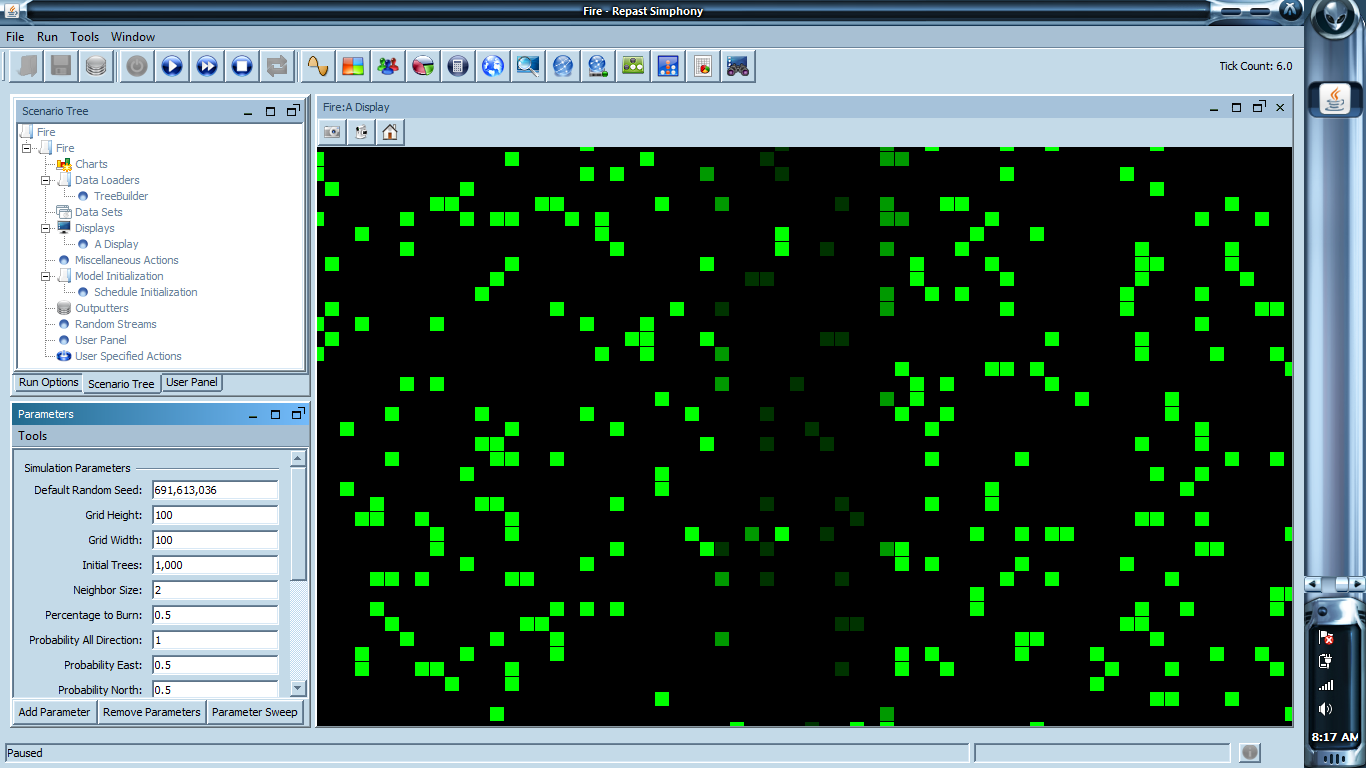
\includegraphics[width=5in]{Images/fire_screen.png}}
\caption{Fire Model}
\label{fig:fire_screen}
\end{center}
\end{figure}


\section{Model Parameters}

After running the fire, set up \emph{Scenario Tree $\rightarrow$ Value Layer Details} with black as the base color and with "Green" color checked.  For the Parameters tab (shown in Figure ~\ref{fig:fire_param}), the descriptions are shown as follow:

\begin{figure}[h]
\begin{center}
\vspace{.2in}
\centerline {
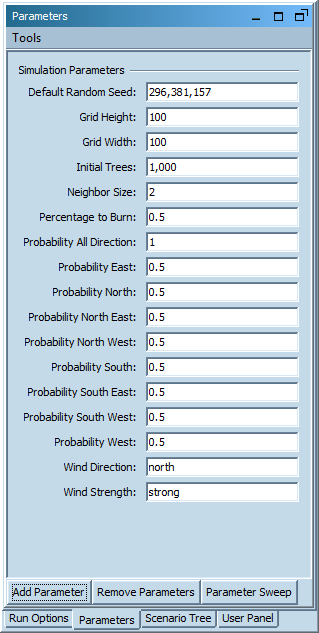
\includegraphics[width=3in]{Images/fire_param.png}}
\caption{Fire Model Parameters}
\label{fig:fire_param}
\end{center}
\end{figure}

\begin{itemize}
\item Grid Height:  Number of rows.
\item Grid Width:  Number of columns.
\item Initial Trees:  Number of trees to populate initially.
\item Neighbor Size:  How far a fire can reach.
\item Percentage to Burn:  Percentage of trees within neighborhood to burn.
\item Probability All Direction:  Apply same probability in all eight directions.  Set to 0 for individual directions (see following eight parameters). 
\item Probability East:  Probability applied towards east direction.
\item Probability North:  Probability applied towards north direction.
\item Probability North East:  Probability applied towards north-east direction.
\item Probability North West:  Probability applied towards north-west direction.
\item Probability South:  Probability applied towards south direction.
\item Probability South East:  Probability applied towards south-east direction.
\item Probability South West:  Probability applied towards south-west direction.
\item Probability West:  Probability applied towards west direction.
\item Wind Direction:  Wind can blow in one of the eight directions.
\item Wind Strength:  Wind strength determines the burn probability of of a tree (strong=0.9, medium=0.5, weak=0.1, none=0.0). 
\end{itemize}
\vspace{.2in}

\section {References}

\begin{itemize}
\item NetLogo's fire model: \emph{http://ccl.northwestern.edu/netlogo/models/Fire}
\item Fire!, Probability, and Chaos: \emph{http://www.shodor.org/interactivate/ lessons/FireProbabilityChaos/}
\end{itemize}

\end{document}  